\usetikzlibrary{arrows,shapes,positioning,shadows,trees,arrows.meta}
\usetikzlibrary{decorations.pathmorphing} % Pour obtenir des lignes de coupes aléatoires
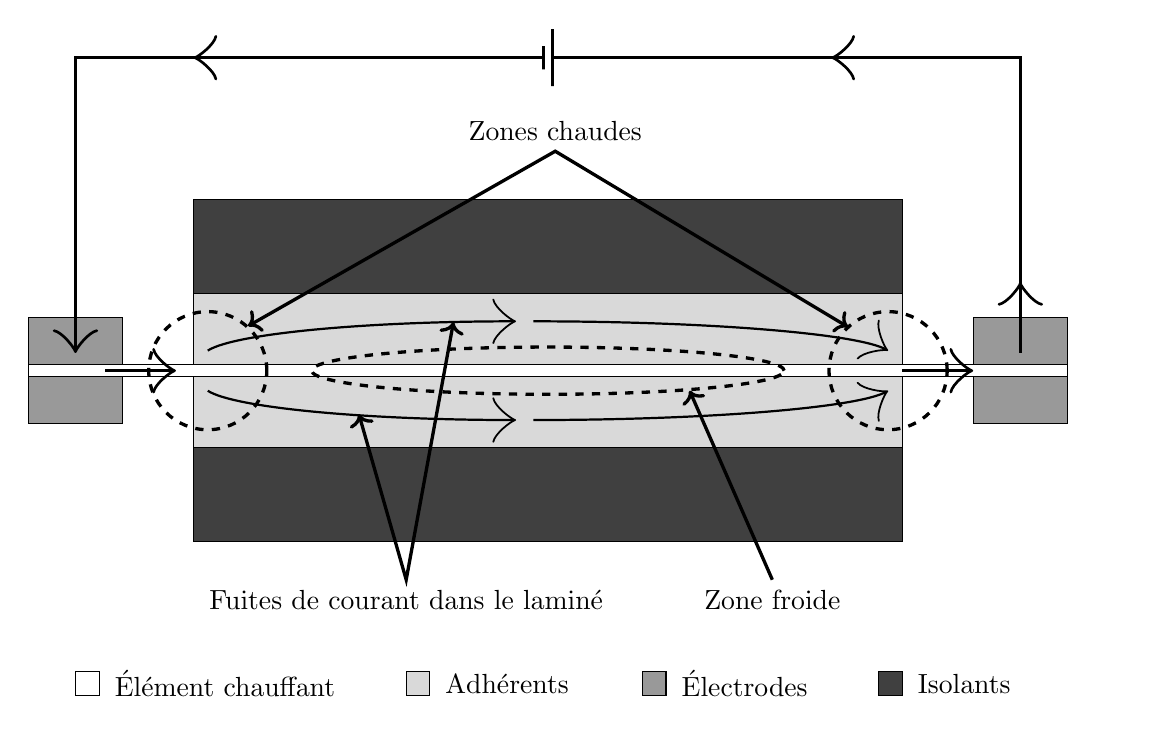
\begin{tikzpicture}[scale=0.6]


%Dimentions du bloc de connection
\def \largconnection{2}
\def \hconnection{1.}

%Distance entre les deux blocs
\def \distance_connection{20}

%Épaisseur de l'élément résistif
\def \tele{0.25}

%Distance entre les blocs de connection et l'isolant
\def \gap{1.5}

%Dimensions des adhérent
\def \tcomp{1.5}

%Épaisseur de l'isolant
\def \tbloc{2}

%Position et taille des annotations
\def \hsource{3.5}
\def \legende{0.5}
\def \distcotation{0.125}

%Couleurs
\def \colinsulator{blue!50}
\def \coladherend{green!50}
\def \colconnector{orange!60}
\def \colresistive{gray!50}

\def \colinsulator{black!75}
\def \coladherend{black!15}
\def \colconnector{black!40}
\def \colresistive{black!0}

%Bloc de pression inferieur
\draw[black,fill=\colinsulator] (\largconnection+\gap,-\tcomp-\tele-\tbloc) -- ++(0,\tbloc) -- ++(\distance_connection-\gap-\gap-\largconnection,0) -- ++(0,-\tbloc) -- cycle; %Face du devant

%Adherant inferieur
\draw[black,fill=\coladherend] (\largconnection+\gap,-\tele-\tcomp) -- ++(0,\tcomp) -- ++(\distance_connection-\gap-\gap-\largconnection,0) -- ++(0,-\tcomp) -- cycle; %Face du devant

%Connection gauche inferieur
\draw[black, fill=\colconnector] (0,-\tele-\hconnection)--++(\largconnection,0)--++(0,\hconnection)--++(-\largconnection,0)--cycle; %Face du devant


%Connection droite inferieur
\draw[black, fill=\colconnector] (\distance_connection,-\tele-\hconnection,0)--++(\largconnection,0,0)--++(0,\hconnection,0)--++(-\largconnection,0,0)--cycle; %Face du devant


%Element chauffant
\draw[black,fill=\colresistive] (0,0,0) -- (\largconnection+\distance_connection,0,0) -- ++(0,-\tele,0) -- (0,-\tele,0) -- cycle; %Face du devant


%Adherant superieur
\draw[black,fill=\coladherend] (\largconnection+\gap,0,0) -- ++(0,\tcomp,0) -- ++(\distance_connection-\gap-\gap-\largconnection,0,0) -- ++(0,-\tcomp,0) -- cycle; %Face du devant


%Connection gauche superieure
\draw[black, fill=\colconnector] (0,0,0)--(\largconnection,0,0)--++(0,\hconnection,0)--(0,\hconnection,0)--cycle; %Face du devant

%Connection droite superieure
\draw[black, fill=\colconnector] (\distance_connection,0,0)--++(\largconnection,0,0)--++(0,\hconnection,0)--++(-\largconnection,0,0)--cycle; %Face du devant

%Bloc de pression superieur
\draw[black,fill=\colinsulator] (\largconnection+\gap,\tcomp,0) -- ++(0,\tbloc,0) -- ++(\distance_connection-\gap-\gap-\largconnection,0,0) -- ++(0,-\tbloc,0) -- cycle; %Face du devant


%Connection de la source de puissance
\draw [very thick] (0.5*\largconnection,\hconnection) -- ++(0,\hsource+\tbloc) -- ++(0.5*\distance_connection-0.1,0) -- ++(0,-0.25) -- ++(0,0.5);
\draw [very thick] (0.5*\largconnection+\distance_connection,\hconnection) -- ++(0,\hsource+\tbloc) -- ++ (-0.5*\distance_connection+0.1,0) -- ++(0,-0.6) -- ++ (0,1.2);


%Courant dans le laminé
\draw[thick, -{Classical TikZ Rightarrow[length=3mm]} ] (\largconnection+1.2*\gap,0.2*\tcomp) arc (170 : 90 : {0.5*\distance_connection-2.25*\gap} and 0.75);
\draw[thick, -{Classical TikZ Rightarrow[length=3mm]} ] (\largconnection+1.2*\gap,-0.2*\tcomp-\tele) arc (-10 : -90 : -{0.5*\distance_connection+2.25*\gap} and 0.75);
\draw [thick, {Classical TikZ Rightarrow[length=3mm]}- ] (\distance_connection-1.2*\gap,0.2*\tcomp) arc (10 : 90 : {0.25*\distance_connection+1.75*\gap} and 0.75);
\draw [thick, {Classical TikZ Rightarrow[length=3mm]}- ] (\distance_connection-1.2*\gap,-0.2*\tcomp-\tele) arc (-10 : -90 : {0.25*\distance_connection+1.75*\gap} and 0.75);
\draw [very thick, {Classical TikZ Rightarrow[length=3mm]}- ] (0.5*\largconnection,0.25*\hconnection) -- ++(0,1.5);
\draw [very thick, -{Classical TikZ Rightarrow[length=3mm]}] (0.5*\largconnection+\distance_connection,0.25*\hconnection) -- ++(0,1.5);
\draw [very thick, -{Classical TikZ Rightarrow[length=3mm]}] (\largconnection-0.25*\gap,-0.5*\tele) -- ++(1*\gap,0);
\draw [very thick, -{Classical TikZ Rightarrow[length=3mm]}] (\distance_connection-1*\gap,-0.5*\tele) -- ++(1.*\gap,0);
\draw [very thick, -{Classical TikZ Rightarrow[length=3mm]}] (\distance_connection-1*\gap,\hconnection+\hsource+\tbloc) -- ++(-\gap,0);
\draw [very thick, -{Classical TikZ Rightarrow[length=3mm]}] (\largconnection+2*\gap,\hconnection+\hsource+\tbloc) -- ++(-1.*\gap,0);

%Identification des fuites de courant
\draw [very thick,<->]  (0.35*\distance_connection,-\tele-0.8) -- ++(1,-3.5) node[below, text width=9cm, align=center] {{Fuites de courant dans le laminé}} --(0.45*\distance_connection,\tcomp-0.6) ;

% zones chaudes
\begin{scope}[radius=1.25, very thick, dashed]
\draw (\largconnection+\gap+0.3,-0.5*\tele) circle ;
\draw (-\gap+\distance_connection-0.3,-0.5*\tele) circle ;
\end{scope}
\draw [very thick,<->]  (\largconnection+\gap+1.155,0.82) -- ++(6.5,3.7) node[above, text width=9cm, align=center] {{Zones chaudes}} --(-\gap+\distance_connection-1.15,\tcomp-0.7) ;

% zone froide
\draw [very thick, dashed] (0.5*\distance_connection+0.5*\largconnection,-0.5*\tele) ellipse [x radius=5,y radius=0.5] ;
\draw [very thick,<-]  (0.7*\distance_connection,-\tele-0.3) -- ++(1.75,-4) node[below, text width=9cm, align=center] {{Zone froide}} ;

%Legende
\begin{scope}[yshift=-12.cm, xshift=1cm]

\begin{scope}[xshift=12cm]
\draw [black, fill=\colconnector] (0,2.5*\tbloc) rectangle ++(\legende,\legende);
\draw (1.25*\legende,2.5*\tbloc+0.5*\legende) node[right]{Électrodes} ;
\end{scope}

\begin{scope}[xshift=7cm]
\draw [black, fill=\coladherend] (0,2.5*\tbloc) rectangle ++(\legende,\legende);
\draw (1.25*\legende,2.5*\tbloc+0.5*\legende) node[right]{Adhérents} ;
\end{scope}

\begin{scope}[xshift=0cm]
\draw [black, fill=\colresistive] (0,2.5*\tbloc) rectangle ++(\legende,\legende);
\draw (1.25*\legende,2.5*\tbloc+0.5*\legende) node[right]{Élément chauffant} ;
\end{scope}

\begin{scope}[xshift=17cm]
\draw [black, fill=\colinsulator] (0,2.5*\tbloc) rectangle ++(\legende,\legende);
\draw (1.25*\legende,2.5*\tbloc+0.5*\legende) node[right]{Isolants} ;
\end{scope}

\end{scope}
\end{tikzpicture}
